\subsection{Round-Robin (RR)}
RR es un algoritmo de los más viejos, simple, justo y ampliamente usado.\newline

A cada proceso se le asigna un tiempo (quantum) durante el cuál le es permitido correr.
Si el proceso sigue corriendo al final del quantum, los recursos le son quitados y se le da paso a otro proceso.
Si el proceso se bloquea, pierde el quantum que le quedaba y los recursos son dados a otro proceso.\newline

Implementar RR es simple, sólo se requiere una lista de procesos 'Ready'.\newline
Cuando el proceso usa su quantum es puesto al final de la lista. \newline
Si éste se bloquea, es removido de dicha lista y volverá a ser agregado en cuanto se desbloquee.

En nuestro caso usamos las siguientes estructuras de datos:
 \begin{description}
  \item[Cola de procesos 'Ready']{}
 \end{description}

\begin{algorithm}
 \caption{Round-Robin}
 \begin{algorithmic}[1] 
 \Procedure{load}{$pid$}
   \State{encolo la nueva tarea en readyTasks}
 \EndProcedure
\newline

 \Procedure{unblock}{$pid$}
   \State{encolo la tarea desbloqueada en readyTasks}
 \EndProcedure
\newline

 \Procedure{tick}{$cpu,\ motivo$}
   \If{el cpu esta ejecutando IDLE}
      \State{llamo a NEXT(cpu) para obtener la próxima tarea a ejecutar}
   \Else
      \If{el motivo es un TICK}
	 \State{Actualizo el quantum}
	 \If{se termino el quantum}
	    \State{encolo la tarea en readyTasks}
	    \State{renuevo el quantum}
	    \State{llamo a NEXT(cpu) para obtener la próxima tarea a ejecutar}
	 \EndIf	    
      \ElsIf{el motivo es un BLOCK o un EXIT}
	  \State{renuevo el quantum}
	  \State{llamo a NEXT(cpu) para obtener la próxima tarea a ejecutar}	
      \EndIf
   \EndIf
 \EndProcedure
\newline
 
 \Procedure{next}{$cpu$}
    \If{hay tareas esperando en readyTasks}
	\State{retornar la primera de la cola readyTasks y quitarla}
    \EndIf
 \EndProcedure
 \end{algorithmic}
\end{algorithm}

Para las simulaciones mantuvimos los siguientes costos:
\begin{description}
 \item[costo de cambio de contexto = 1 :]{En un CPU real se deben intercambiar estructuras de datos que contienen información de los procesos antes de poder correr la nueva tarea.}
 \item[costo de migración de núcleo = 2 :]{Se deben intercambiar las mismas estructuras de datos que para el cambio de contexto pero la 'distancia' del caché de un núcleo al de otro es mayor que dentro de sí mismo.}
\end{description}

Correremos un lote de tareas para verificar que el comportamiento del scheduler es el esperado.

\begin{center}
 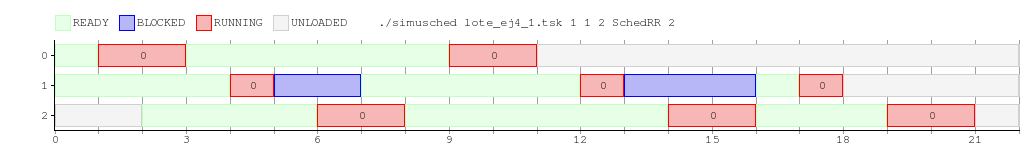
\includegraphics{./RR/RR_simple.png}
\end{center}

Tenemos tres tareas, la segunda realiza llamadas bloqueantes.
-Se cargan a la cola las tareas 1 y 2. Cola: 1-2
-Se ejecuta 1, se carga 3 a la cola. Cola: 2-3 (La tarea 1 está corriendo, por lo tanto está fuera de la lista).
-Se acaba el quantum de 1, vuelve a la lista y se ejecuta el primero de la cola, 2. Cola 3-1
-La tarea 2 realiza una llamada bloqueante, se ejecuta la siguiente en la cola. Cola: 1
-Mientras se ejecuta 3, se desbloquea la tarea 2 y vuelve a la lista. Cola: 1-2
-Se ejecuta 1, termina, y se carga 2. Cola: 3
-A partir de este momento quedan solamente 2 y 3 que se alternan hasta completar su ejecución.


%Análisis de casos particulares:
%A continuación presentamos el comportamiento del scheduler para cierto lote de tareas, variando el quantum otorgado.
%En el primero, consideramos un quantum mínimo, de un ciclo, en el segundo uno de 4, y el último de 11.